%----------------------------------------------------------------------------------------
\chapter{Monte-Carlo methods}
\label{sec:monte:carlo}
\index{Monte Carlo Method}
%----------------------------------------------------------------------------------------
Monte Carlo methods are computational algorithms which rely on repeated random sampling to obtain numerical results. The principle is to use randomness to solve the problem because it is difficult or impossible to use other approaches. When this method was developed in the 1940s by Ulam and von Neumann they called the method "Monte Carlo" in reference to the Monte Carlo Casino in Monaco where Ulam's uncle gambled. Today Monte Carlo methods are widely used in the following three problem classes:
\begin{itemize}
\item Optimization,
\item Numerical integration, and
\item Probability distributions.
\end{itemize}
For the importance of the method we refer to~\cite{kroese2014monte}, and for more details about Monte Carlo Methods we refer to~\cite{shonkwiler2009explorations}.\\

Let us look into the computational aspects of the Monte Carlo methods. Independent of the problem class, a general pattern is observed:
\begin{enumerate}
\item Define the input parameters,
\item Randomly chose input parameters,
\item Do deterministic computations on the inputs,
\item Aggregate the results\text{.}
\end{enumerate}

\begin{figure}[h]
  \begin{center}
  \begin{tikzpicture}
\draw (0,0) -- (2,0) -- (2,2) -- (0,2) -- cycle;
\draw[fill=cadetgrey, opacity=0.5] (1,1) circle (1cm);
\draw[->] (1,1) -- (2,1);
\draw[fill=black] (1,1) circle (0.05cm);
\node[above] at (1.5,1) {\small $r=\sfrac{1}{2}$};
\draw[<->] (0,-0.35) -- (2,-0.35);
\node[below] at (1,-0.35) {\small $1$};
\draw[<->] (-0.35,0) -- (-0.35,2);
\node[left] at (-0.35,1) {\small $1$};
\end{tikzpicture}
  \end{center}
  \caption{Sketch of the geometry used within the Monte Carlo method to estimate the value of $\pi$.}
  \label{fig:monte}
\end{figure}
To understand these four steps, we will compute the value of $\pi$ using a Monte Carlo method. Figure~\ref{fig:monte} sketches the first two ingredients: a unit square and a circle. First, a unit square is defined as $1 \times 1$, which means it has a side length of 1. The area $A_s$ is therefore also $1. Second, the circle with radius $r=\sfrac{1}{2}$ is drawn at the center of the unit square. The area of the circle is $A_c=\pi r^2$. Using the radius $r=\sfrac{1}{2}$ the area is $A_c=\pi(\sfrac{1}{2})^2=\sfrac{\pi}{4}$. Now, since we have defined the area of the circle and the square, we can use them to estimate the value of $\pi$:
\begin{align}
A_c &= \sfrac{\pi}{4} \notag\\
\pi &= 4 A_c \notag\\
\pi &= 4 \sfrac{A_c}{A_s}\text{.}
\end{align}
Note that the operation on the first equation is a multiplication by four. Going from the second line to the third line, we use the fact that the area of the square is one. \\

Now, we can estimate $\pi$ by the general pattern described above.
\begin{itemize}
\item \textbf{Define the input parameters}: \\ A coordinate  $(x,y)\in\mathbb{R}$ in the domain of the unit square $[0,1]\times [0,1]$
\item\textbf{ Randomly chose input parameters}:\\ We randomly draw $N$ values for $x$ and $y$ in the range of $[0,1]$
\item \textbf{Do deterministic computations on the inputs}:  \\
We must validate if the coordinate $(x,y)$ is inside the circle or not with the inequality $x^2+y^2\leq 1$. If the coordinate is within the circle, we increment $N_C$.
\item \textbf{Aggregate the results}: \\
We compute $\pi\approx \sfrac{4N_c}{N}$
\end{itemize}
\vspace{0.25cm}

Figure~\ref{fig:algorithm:monte} shows the flow chart of the algorithm for estimating $\pi$ using the Monte Carlo method. First, the decision if the current draw of the random number is less than the desired total amount of random numbers $N$. If we have not yet drawn enough random numbers, we have to guess two random numbers $x$ and $y$ (see Section~\ref{sec:random:numbers} for how to generate random numbers in C++). Next, we have to check if the drawn coordinate $(x,y)$ is within the circle. If so, we increment the count of the number of points that have landed within the circle $N_c$. We have to repeat these steps until $i>N$. Once we have drawn enough random numbers, we can compute $\pi\approx\sfrac{4N_c}{N}$ and finish the program.\\

\begin{figure}[tb]
    \centering
	\begin{tikzpicture}[node distance=1.125cm, scale=0.75, transform shape]
	\node (start) [startstop] {Start}; 
	\node (dec1) [decision, below of=start , yshift=-1.cm] { $i < N$};
	\node (n0) [process, below of=dec1,yshift=-1.cm] {Draw random number $x$ and $y$};
	\node (dec2) [decision, below of=n0 , yshift=-1.cm] { $x^2 + y^2 < 1$};
	\node (n1) [process, below of=dec2,yshift=-1.cm] {Increment $N_C$};
	\node (n2) [process, below of=n1,yshift=-1.cm] {Increment $i$};
	\node (n2) [process, below of=n1,yshift=-1.cm] {Increment $i$};
	\node (n3) [process, right of=dec1,xshift=2.5cm] {Compute $\sfrac{4N_c}{N}$};
	\node (stop) [startstop, right of=dec1, xshift=6.cm] {Finished}; 
	%lines
	\draw [->] (start) -- (dec1);
	\draw [->] (dec1) -- (n0);
	\draw [->] (n0) -- (dec2);
	\draw [->] (n1) -- (n2);
	\draw [->] (n3) -- (stop);
	%dec1
	\draw [->] (dec1) -- node[anchor=north] {no} (n3);
	\draw [->] (dec1) -- node[anchor=west] {yes} (n0);	
	\draw [->] (dec2) -- node[anchor=west] {yes} (n1);	
	\draw [->] (n2.west) -- ++(-3.0,0) -- ++(0,8.5) -- ++(3.5,0);
	\draw [->] (dec2)  -- ++(-4.5,0) ;
	\end{tikzpicture}
	\caption{Flow chart for the Monte Carlo method to estimate $\pi$.}
	\label{fig:algorithm:monte}
\end{figure}

Next,let us ask the question, "What is a good choice for $N$ to get a good approximation of $pi$?" Figure~\ref{fig:monte:carlo:samples} shows the distribution of the point inside the circle (\textcolor{amaranth}{red}) and outside of the circle (\textcolor{azure}{blue}) for $N=10$, $N=100$, and $N=1000$ random numbers. One can see that a certain amount of random numbers is needed to have enough samples inside and outside of the circle. Figure~\ref{fig:monte:carlo} shows the absolute error in percent for various amounts of random numbers. One can see that with a thousand random numbers the accuracy is quite reasonable. 


\begin{figure}[bt]
\begin{subfigure}{.3\textwidth}
  \centering
\def\x{0}
\def\y{0}
\def\k{0}
\def\radius{4}
\begin{tikzpicture}
    \draw[fill=cadetgrey, opacity=0.1] (\radius,0) arc(0:90:\radius) -- (0,0) -- cycle;
    \draw[gray, opacity=0.25] (0,0) rectangle (\radius,\radius);
    \draw[->] (0,0) -- (1.1*\radius,0);
    \draw[->] (0,0) -- (0,1.1*\radius);
    \foreach \i in {1,2,...,10}{%
        \pgfmathsetmacro\x{\radius*rnd}%
        \pgfmathsetmacro\y{\radius*rnd}%
        \pgfmathsetmacro\k{(pow(\x,2)+pow(\y,2)) <pow(\radius,2)}%
        \pgfmathparse{ifthenelse(\k==1,"amaranth","azure")}%
        \fill[\pgfmathresult] (\x,\y)circle(0.75pt);%
    }
\end{tikzpicture}
  \caption{$N=10$}
  \label{fig:sub-first}
\end{subfigure}
\hfill
\begin{subfigure}{.3\textwidth}
  \centering
\def\x{0}
\def\y{0}
\def\k{0}
\def\radius{4}
\begin{tikzpicture}
    \draw[fill=cadetgrey, opacity=0.1] (\radius,0) arc(0:90:\radius) -- (0,0) -- cycle;
    \draw[gray, opacity=0.25] (0,0) rectangle (\radius,\radius);
    \draw[->] (0,0) -- (1.1*\radius,0);
    \draw[->] (0,0) -- (0,1.1*\radius);
    \foreach \i in {1,2,...,100}{%
        \pgfmathsetmacro\x{\radius*rnd}%
        \pgfmathsetmacro\y{\radius*rnd}%
        \pgfmathsetmacro\k{(pow(\x,2)+pow(\y,2)) <pow(\radius,2)}%
        \pgfmathparse{ifthenelse(\k==1,"amaranth","azure")}%
        \fill[\pgfmathresult] (\x,\y)circle(0.75pt);%
    }
\end{tikzpicture}
  \caption{$N=100$}
\end{subfigure}
\hfill
\begin{subfigure}{.3\textwidth}
  \centering
\def\x{0}
\def\y{0}
\def\k{0}
\def\radius{4}
\begin{tikzpicture}
    \draw[fill=cadetgrey, opacity=0.1] (\radius,0) arc(0:90:\radius) -- (0,0) -- cycle;
    \draw[gray, opacity=0.25] (0,0) rectangle (\radius,\radius);
    \draw[->] (0,0) -- (1.1*\radius,0);
    \draw[->] (0,0) -- (0,1.1*\radius);
    \foreach \i in {1,2,...,1000}{%
        \pgfmathsetmacro\x{\radius*rnd}%
        \pgfmathsetmacro\y{\radius*rnd}%
        \pgfmathsetmacro\k{(pow(\x,2)+pow(\y,2)) <pow(\radius,2)}%
        \pgfmathparse{ifthenelse(\k==1,"amaranth","azure")}%
        \fill[\pgfmathresult] (\x,\y)circle(0.75pt);%
    }
\end{tikzpicture}
  \caption{$N=1000$}
  \label{fig:sub-second}
\end{subfigure}
\caption{Distribution of the points inside the circle (\textcolor{amaranth}{red}) and outside of the circle (\textcolor{azure}{blue}) for $N=10$, $N=100$, and $N=1000$ random numbers.}
\label{fig:monte:carlo:samples}
% This example was adapted from https://tex.stackexchange.com/questions/244488/monte-carlo-method-drawing
\end{figure}


\begin{figure}[tb]
\centering
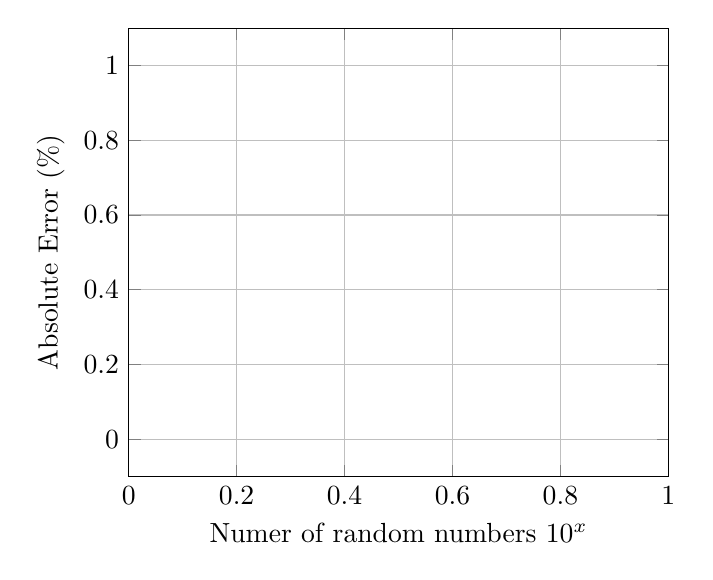
\begin{tikzpicture}
\begin{axis}
[
	xmin=0,   xmax=4,
	grid=major,
	xlabel=Numer of random numbers $10^x$,
	ylabel=Absolute Error (\%)
]
\montecarlo{10}{1}
\montecarlo{100}{2}
\montecarlo{1000}{3}
\end{axis}
\end{tikzpicture}
\caption{The absolute error for various amounts of random numbers. One can see that with a thousand random numbers the accuracy is quite reasonable. }
\label{fig:monte:carlo}
\end{figure}

\begin{exercise}
Make a list of which C++ features we need to implement the flow chart in Figure~\ref{fig:algorithm:monte}.
\end{exercise}

\begin{exercise}
Implement the Algorithm in Figure~\ref{fig:algorithm:monte} using the random numbers in Section~\ref{sec:random:numbers}.
\end{exercise}


%----------------------------------------------------------------------------------------
\chapter{$N$-body problems}
\index{$N$-body problems}
\label{sec:nbody}
%----------------------------------------------------------------------------------------
The $N$-body problem is the physics problem of predicting the individual motions of members of a group of celestial objects interacting with each other gravitationally. We want to predict the interactive forces and the motion of all celestial bodies at all future times. We assume that we know their orbital properties, \emph{e.g.}\ the initial positions, velocity, and time.\\

Before we look into the $N$-body problem, let us step back and look at the two-body problem. Let us look at two gravitational bodies with the masses $m_i$ and $m_j$ and the positions $\mathbf{r}_i,\mathbf{r}_j\in\mathbb{R}^3$. To define the equation of motion, we refer to the following definitions:
\vspace{0.25cm}
\begin{enumerate}
\item \textbf{The Law of Gravitation}: \\
The force of $m_i$ acting on $m_j$ is 
\begin{align}
\mathbf{F}_{ij}= G m_i m_j \frac{\mathbf{r}_j-\mathbf{r}_2}{\vert \mathbf{r}_1-\mathbf{r}_i \vert^3} (See Figure~\ref{fig:nbody:motion})
\end{align}
The universal constant of gravitation $G$ was estimated as $6.67408\cdot 10^{-11}m^3kg^{-1}s^{-2}$ in 2014~\cite{mohr2016codata}.
\item \textbf{Velocity and acceleration}: 
\begin{enumerate}
\item The velocity of $m_i$ is
\begin{align}
\mathbf{v}_i = \frac{d \mathbf{r}_i}{dt} \label{eq:nbody:vel}
\end{align}
\item The acceleration of $m_i$ is
\begin{align}
\mathbf{a}_i = \frac{d \mathbf{v}_i}{dt} \label{eq:nbody:acc}
\end{align}
\end{enumerate}
For more details about vectors and basic vector operations, we refer to Section~\ref{sec:linalg:vectors}.
\item \textbf{The second Law of Mechanics}:  (Force is equal to mass times acceleration) 
\begin{align}
\mathbf{F}= m \mathbf{a} \label{eq:law:first}
\end{align}
\end{enumerate}
With these three definitions, we can derive the equation of motion for the first body as follows:
\begin{align}
\mathbf{F}_{ij}&=G m_i m_j \frac{\mathbf{r}_j-\mathbf{r}_i}{\vert \mathbf{r}_j-\mathbf{r}_i \vert^3} \label{eq:nbody:motion1} \\
m_i \mathbf{a}_i &= G m_i m_j \frac{\mathbf{r}_j-\mathbf{r}_i}{\vert \mathbf{r}_i-\mathbf{r}_j \vert^3} \label{eq:nbody:motion2} \\
\frac{d \mathbf{v}_i}{dt} & = G m_j \frac{\mathbf{r}_j-\mathbf{r}_i}{\vert \mathbf{r}_j-\mathbf{r}_i \vert^3} \label{eq:nbody:motion3} \\
\frac{d^2 \mathbf{r}_i}{dt^2} & = G m_j \frac{\mathbf{r}_j-\mathbf{r}_i}{\vert \mathbf{r}_j-\mathbf{r}_i \vert^3}
\label{eq:nbody:motion4}
\end{align}
To get from Equation~\eqref{eq:nbody:motion1} to Equation~\eqref{eq:nbody:motion2}, we substitute $\mathbf{F}_{ij}$ with $m_i \mathbf{a}_i$ using Equation~\ref{eq:law:first}.  From Equation~\eqref{eq:nbody:motion2} to Equation~\eqref{eq:nbody:motion3}, we divide by $m_i$ and replace $\mathbf{a}_i$ according to Equation~\ref{eq:nbody:acc}. From Equation~\eqref{eq:nbody:motion3} to Equation~\eqref{eq:nbody:motion4}, we substitute Equation~\ref{eq:nbody:vel}. Note that we used Newton's law of universal gravitation~\cite{newton1833philosophiae}.\\


\begin{figure}[tb]
\centering
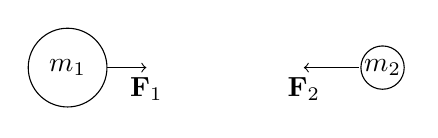
\begin{tikzpicture}
\draw (-2,0) circle (0.5cm);
\draw (2,0) circle (0.275cm);
\node at (-2,0) {$m_1$};
\node at (2,0) {$m_2$};
\draw[->] (-1.5,0)--(-1,0);
\draw[->] (1.7,0)--(1,0);
\node[below] at (-1,0) {$\mathbf{F}_1$};
\node[below] at (1,0) {$\mathbf{F}_2$};
\end{tikzpicture}
\caption{Sketch of the two celestial bodies with the masses $m_1$ and $m_2$ and the gravitational interaction forces $\mathbf{F}_1$ and $\mathbf{F}_1$. Equation~\ref{eq:nbody:motion4} shows the equation of motion for the two-body system.   }
\label{fig:nbody:motion}
\end{figure}

Now we formulate the problem for $n$ bodies, assuming that the force at one body is equal to the sum over all bodies, excepting itself.
\begin{align}
\mathbf{F}_i = \sum\limits_{j=1,i\neq j}^n \mathbf{F}_{ij} = \sum\limits_{j=1,,i\neq j}^n G  m_j \frac{\mathbf{r}_j - \mathbf{r}_i}{\vert \mathbf{r}_j - \mathbf{r}_i\vert^3} \text{.} \label{eq:nbody:motion}
\end{align}
These are the laws of conservation for the $N$-body problem:
\begin{enumerate}
\item Linear Momentum: $\sum\limits_{i=1}^n m_i \mathbf{v}_i = M_0$
\item Center of Mass: $\sum\limits_{i=1}^n m_i \mathbf{r}_i = M_0 t + M_1$
\item Angular Momentum: $\sum\limits_{i=1}^n m_i (\mathbf{r}_i \times \mathbf{v}_i) = \mathbf{c}$
\item Energy: T-U=h with \\
$ T = \frac{1}{2} \sum\limits_{i=1}^n m_i \mathbf{v}_i \circ \mathbf{v}_i  , U= \sum\limits_{i=1}^n \sum\limits_{j=1}^n G \frac{m_i m_j}{\vert\mathbf{r}_i - \mathbf{r}_j\vert} $
\end{enumerate}
These laws are just shown for completeness. For more details about the theory and the derivations, we refer to~\cite{aarseth2008cambridge,aarseth2003gravitational}. This text focuses on the implementation details of the $N$-body problem withb C++.


%----------------------------------------------------------------------------------------
\section{Algorithm}
%----------------------------------------------------------------------------------------
Figure~\ref{fig:nbody:algorithm} shows the three steps for the $N$-body simulation. In this section we focus on the implementation details of the first two steps. Equation~\ref{eq:nbody:motion} shows how to compute the force for one celestial object. Recall that the $\sum$ translates to a \cpp{for} loop as we discussed in Section~\ref{sec:iteration:statements}. To compute the forces of all bodies, the so-called nested \cpp{for} loop or direct sum is used. Listing~\ref{code:directsum} shows the concept of the direct sum which is robust, accurate, and completely general. The computational costs per body are $\mathcal{O}(n)$ and the computational costs for all bodies are $\mathcal{O}(n^2)$. The symbol $\mathcal{O}$ is the so-called "Big O" notation, which we use to describe algorithm run time or space requirement growth as the input size grows. In our case the computational cost per body increases linearly, since we have to compute the force $n-1$ times for all particles. The Big O notation $\mathcal{O}(n)$ means that the total computational cost for n computations is less than or equal to $n$. These symbols are defined in the Bachmann–Landau notation\index{Bachmann–Landau notation}~\cite{bachmann1894analytische,landau2000handbuch,knuth1997art}. For all bodies the computational cost increases to the power of two since we have to compute the forces $n-1$ times for all $n$ bodies. The direct sum is feasible for a small number of celestial objects, but for larger numbers the tree-based codes or the Barnes-Hut method~\cite{barnes1986hierarchical} reduce the computational costs to $\mathcal{O}(n\log(n))$. \\

\begin{figure}[tb]
\centering
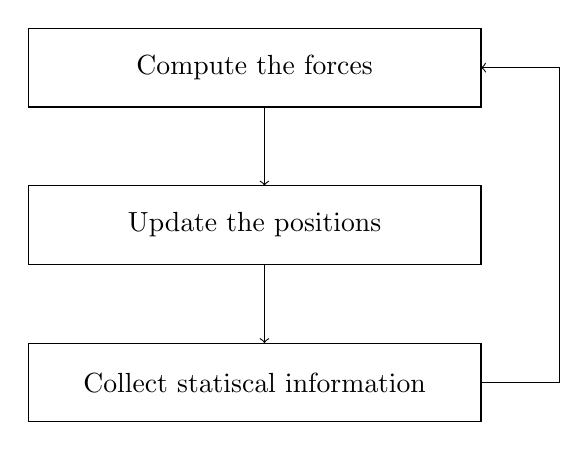
\begin{tikzpicture}
\draw (-3.75,0) rectangle (2,1) node[pos=.5] {Compute the forces};
\draw[->](-0.75,0) -- (-0.75,-1);
\draw (-3.75,-2) rectangle (2,-1) node[pos=.5] {Update the positions};
\draw[->](-0.75,-2) -- (-0.75,-3);
\draw (-3.75,-4) rectangle (2,-3) node[pos=.5] {Collect statiscal information};
\draw[->] (2,-3.5) -- (3,-3.5) -- (3,0.5) -- (2,0.5);
\end{tikzpicture}
\caption{The three steps of the algorithm for the $N$-body simulation. First, the forces for all objects are computed using Equation~\ref{eq:nbody:motion}. Second, the updated positions are computed using Equation~\ref{eq:position:update} and Equation~\ref{eq:position:update2}. Third, the statistical information is evaluated.  }
\label{fig:nbody:algorithm}
\end{figure}


\begin{lstlisting}[language=c++,caption={Example for the direct sum\index{direct sum}.\label{code:directsum}},float,floatplacement=tb]
for(size_t i = 0; i < bodies.size(); i++)
	for(size_t j = 0; j < bodies.size(); j++)
		if ( i != j )
			//Compute forces
\end{lstlisting}

For the second step of the algorithm, we need to update the positions for the evolution of the system over the time $T$. For the discretization in time, we define the following quantities:
\begin{itemize}
\item $\Delta t$ the uniform time step size
\item $t_0$ the beginning of the evolution
\item $T$ the final time of the evolution
\item $k$ the time steps such that $k\Delta t=T$.
\end{itemize}
Next, we need to compute the derivatives to obtain the velocity and the acceleration of each celestial object. One numerical method to approximate the derivation is given by
\begin{align}
u'(x) \approx \frac{u(x+h)-u(x)}{h}
\end{align}
which is the finite difference method. Figure~\ref{fig:nbody:finitedifference} sketches the principle of the finite difference method. For a sufficiently small $h$, we can approximate the derivation at the coordinate $x$. For example: Choosing $h=1$ and $x=3$, we get $u'(x)=\sfrac{(4-3)}{1}=1$ which aligns with $u'(x)=1$ using the analytic derivation of $u(x)$. Now we can use the Euler method to compute the updated positions at time $t_{k+1}$. First we approximate the velocity using the finite difference scheme
\begin{align}
\mathbf{v}_i(t_k) = \frac{d\mathbf{r}_i}{dt} \approx \frac{\mathbf{r}_i(t_{k+1})-\mathbf{r}_i(t_k)}{\Delta t}\label{eq:vel}\text{.}
\end{align}
We do the same for the acceleration
\begin{align}
\mathbf{a}_i(t_k) = \frac{d\mathbf{v}_i}{dt}   \approx  \frac{\mathbf{v}_i(t_k)-\mathbf{v}_i(t_k-1)}{\Delta t} = \frac{\mathbf{F}_i}{m_i}  \label{eq:acc} 
\end{align}
from Equation~\ref{eq:law:first} we get $\mathbf{a}_i=\sfrac{\mathbf{F}_i}{m_i}$. More details~\cite{strikwerda2004finite,leveque2007finite,euler1824institutionum}. With the above approximations the velocity is computed as
\begin{align}
\mathbf{v}_i(t_k) = \mathbf{v}_i(t_{k-1}) + \Delta t \frac{\mathbf{F}_i}{m_i} \label{eq:position:update}
\end{align}
using Equation~\eqref{eq:acc} and the fact that the finite difference approximation of the acceleration is equal to $\sfrac{\mathbf{F}_i}{m_i}$. Finally, the updated position is computed as
\begin{align}
\mathbf{r}_i(t_{k+1}) = \mathbf{r}_{t_k} + \Delta t \mathbf{v}_i(t_k)  \label{eq:position:update2}
\end{align} 
using Equation~\eqref{eq:vel}. Note that we used easy methods to update the positions, but more sophisticated methods, \emph{e.g.}\ Crank--Nicolson method~\cite{crank1947practical}, are available

\begin{exercise}
Look at the equations in this section and try to derive the Equation~\ref{eq:position:update} and Equation~\ref{eq:position:update} on your own.
\end{exercise}

\begin{exercise}
Implement the $N$-body problem using the template code\link{https://github.com/diehlpkteaching/N-Body} on GitHub.
\end{exercise}

\begin{figure}[tb]
\centering
\begin{tikzpicture}
\begin{axis}[
        xmin=0, xmax=6, % x scale
        ymin=0, ymax=6, % y scale
]
\addplot[azure,thick]    {x};
\legend{$u(x)$}
\addplot[amaranth, mark=*] coordinates{(3,3)} node[midway,above left,amaranth] {$u(x)$};
\addplot[amaranth,  mark=*] coordinates{(4,4)} node[midway,above left,amaranth] {$u(x+h)$};
\addplot +[mark=none,cadetgrey] coordinates {(3, 3) (4, 3)};
\addplot +[mark=none,cadetgrey] coordinates {(4, 3) (4, 4)};
\addplot[cadetgrey,  mark=none] coordinates{(3.5,3)} node[midway,below] {$h$};
\end{axis}
\end{tikzpicture}
\caption{The principle of the finite difference method. For a sufficiently small $h$, we can approximate the derivation at the coordinate $x$. For example: Choosing $h=1$ and $x=3$, we get $u'(x)=\sfrac{(4-3)}{1}=1$ which aligns with $u'(x)=1$ using the analytic derivation of $u(x)$. Now we can use the Euler method to compute the updated positions at time $t_{k+1}$.}
\label{fig:nbody:finitedifference}
\end{figure}

%----------------------------------------------------------------------------------------
\chapter{Peridynamics}
\label{sec:pd}
%----------------------------------------------------------------------------------------
Peridynamic, a alternative formulation of continuum mechanics with a focus on discontinuous displacement as they arise in fracture mechanics, was introduced by Silling in 2000~\cite{silling2000reformulation,silling2005meshfree}. Models crack and fractures on a mesoscopic scale using Newton's second law (force equals mass times acceleration)
\begin{align}
F = m \cdot a = m \cdot \ddot X \text{.}
\end{align}



%----------------------------------------------------------------------------------------
\section{Brief introduction in classical continuum mechanics}
%----------------------------------------------------------------------------------------
We briefly look into the ingredients of classical continuum mechanics which are needed to introduce peridynamics. In Figure~\ref{fig::chapter2:01} on the lift-hand side, we see the continuum in the reference configuration $\Omega_0 \subset \R^3$ which is the state where we have no internal forces and we are in the equilibrium. We denote these positions with capitalized $X \in \R^3$ to distinguished with the new position after the deformation $\phi : \Omega_0 \rightarrow \R^3$. The deformation implied for example by some external forces moves the continuum from the reference configuration  $\Omega_0$ to the current configuration $\Omega(t)$. The new position of $X$ is now $x(t,X)$.\\

Let us look more closely in the definitions above. The deformation $\phi:[0,T]\times\R^3\rightarrow\R^3$ of a material point $X$ in the reference configuration $\Omega_0$ to the so-called current configuration $\Omega(t)$ is given by
\begin{align*}
\phi(t,X) := id(X) + u(t,X) = x(t,X) \text{,}
\end{align*}
where $u:[0,T]\times\R^3\rightarrow\R^3$ refers to the displacement
\begin{align*}
u(t,X):= x(t,X) - X\,\text{.}
\end{align*}
The stretch $s:[0,T]\times\R^3\times\R^3\rightarrow\R^3$ between the material point $X$ and the material point $X'$ after the deformation $\phi$ in the configuration $\Omega(t)$ is defined by
\begin{align*}
s(t,X,X') := \phi(t,X') - \phi(t,X) \,\text{.}
\end{align*}
We just covered the prerequisites of classical continuum mechanics which are necessary to introduce the peridynamic theory. For more details, we refer to~\cite{gurtin1982introduction,liu2013continuum}.

\begin{figure}[tb]
\centering
\begin{tikzpicture}
\draw[fill=blue, opacity=0.5](1,1) circle (1);
 \node at (1,2.35) {{\small $\Omega_0$}};
 \draw[fill=blue,](1,1) circle (0.075);
 \node at (1,0.725) {{\small $X$}};
 \node at (6,1) {
\includegraphics[scale=1.25]{images/deformation.pdf}};
 \node at (6,2.35) {{\small $\Omega(t)$}};
 \draw[fill=blue,](6,0.725) circle (0.075);
 \node at (6,0.45) {{\small $x(t,X)$}};
 \node at (3.75,2.45) {{\small $\phi:\Omega_0\rightarrow \R^3$}};
 \draw [arrow, bend angle=45, bend left] (1.95,1.25) to (5.8,1);
\end{tikzpicture}
\caption[The continuum in the reference configuration $\Omega_0$ and after the deformation $\phi : \Omega_0 \rightarrow \R^3$ in the current configuration $\Omega(t)$ at time $t$.]{The continuum in the reference configuration $\Omega_0$ and after the deformation $\phi : \Omega_0 \rightarrow \R^3$ with $\det(\text{grad}\;\phi) > 0$ in the current configuration $\Omega(t)$ at time $t$.}
\label{fig::chapter2:01}
\end{figure}

%----------------------------------------------------------------------------------------
\section{Brief introduction in bond-based peridynamics}
%----------------------------------------------------------------------------------------
We can use Newton;s second law (force equals mass times acceleration) and formulate it as
\begin{align}
\rho(X)a(t,X):=
\int\limits_{B_\delta(X)} f\left(t,x(t,X')-x(t,X), X'-X\right)dX' + b(t,X)\,\text{,}
\label{eq::chapter2:01}
\end{align}
to compute the acceleration $a:\ftime\times\R^3\rightarrow\R^3$ of a material point at position $X$ at time $t$. With the pair-wise force function $f:[0,T]\times\R^3\times\R^3\rightarrow\R^3$, the mass density $\rho(X)$, and the external force $b:[0,T]\times\mathbb{R}^3\rightarrow\mathbb{R}^3$. Following assumptions are made
\begin{enumerate}
\item The medium is continuous (equal to a continuous mass density field exists)
\item Internal forces are contact forces (equal to that material points only interact if they are separated by zero distance.
\item Conservation laws of mechanics apply
\begin{enumerate}
\item Conservation of mass
\item Conservation of linear momentum
\begin{align*}
f(t,-(x(t,X')-x(t,X)),-(X'-X))= -f(t,x(t,X')-x(t,X), X'-X)
\end{align*}
\item Conservation of angular momentum
\begin{align*}
(x(t,X')-x(t,X)+X'-X) \times f\left(t,x(t,X')-x(t,X), X'-X\right) = 0
\end{align*}
\end{enumerate}
\end{enumerate}

%----------------------------------------------------------------------------------------
\subsection{Material model}
%----------------------------------------------------------------------------------------
There are several material models available, however, we look into the Prototype Microelastic Brittle (PMB) model, since it was one of the first material models. In this model the assumption is made that the pair-wise force $f$ only depends on the relative normalized bond stretch $s:[0,T]\times\mathbb{R}^3\times\mathbb{R}^3\rightarrow\mathbb{R}$
\begin{align}
s(t,x(t,X')&-x(t,X),X'-X):= \\ &\frac{\vert\vert x(t,X')-x(t,X))\vert\vert - \vert\vert X'-X\vert\vert}{\vert\vert X'-X\vert\vert}\,\text{,} 
\end{align}
where $X'-X$ is the vector between the material points in the reference configuration $\Omega_0$ and $x(t,X')-x(t,X)$ is the vector between the material point in the current configuration $\Omega(t)$. As a material property, the so-called stiffness constant $\textcolor{azure}{c}$ is introduced and the pair-wise force function reads as
\begin{align}
f(t,x(t,X')-x(t,X),X'-X):=  \textcolor{blue}{c} \, s(t,x(t,X')-x(t,X),X'-X)\frac{x(t,X')-x(t,X)}{\Vert x(t,X')-x(t,X)\Vert} \text{.}
\end{align}
The pair-wise force function is shown in Figure~\ref{fig::force::sketch}. Which is a linear line with the slope \textcolor{azure}{blue}. Note that we do not have introduced damage to the material model yet. Therefore, a scalar valued history dependent function $\mu:[0,T]\times\mathbb{R}^3\times\mathbb{R}^3\rightarrow\mathbb{N}$ is added to the computation of the pair-wise force
\begin{align}
f(t,x(t,X')-x(t,X),X'-X)&:= \notag\\ & \textcolor{azure}{c} s(t,x(t,X')-x(t,X),X'-X) \notag\\&\mu\args \frac{x(t,X')-x(t,X)}{\Vert x(t,X')-x(t,X)\Vert}\,\text{.} 
\end{align}
with
\begin{align}
\mu(t,x(t,X')&-x(t,X),X'-X):= 
 \left\{
 \begin{aligned}
 & 1 \quad s(t,x(t,X')-x(t,X),X'-X) < \textcolor{azure}{s_{c}} \\
 %& \qquad -\alpha s_\text{smin}(t') \forall 0 \leq t' \leq t
%\\[1ex]
 & 0 \quad \text{otherwise}
\end{aligned}
 \right.
\end{align}
The pair-wise force function with the damage is incorporated is shown in Figure~\ref{fig::force::sketch::critical}.
With the scalar valued history dependent function $\mu$ the notion of damage $d(t,X):[0,T]\times\R^3\rightarrow\R$ can be introduced via
\begin{align}
d(t,X):= 1- \frac{\displaystyle\int\limits_{B_\delta(X)}\mu\args dX'}{\displaystyle\int\limits_{B_\delta(X)}dX'}\,\text{.}
\label{eq::damage:nodal}
\end{align}
To express damage in words, it is the ratio of the active (non-broken) bonds and the amount of bonds in the reference configuration within the neighborhood. Note that we have two material properties the stuffiness constant $\textcolor{blue}{c}$ and the critical stretch $\textcolor{blue}{s_c}$. We can related these to continuum mechanics as
\begin{align}
c = \frac{18K}{\pi\delta} \qquad \text{ and } \qquad s_c = \frac{5}{12} \sqrt{\frac{K_{Ic}}{K^2\delta}}
\end{align}
With $K$ is the bulk modulus and $K_Ic$ is the critical stress intensity factor.



\begin{figure}[bt]
\begin{subfigure}{.45\textwidth}
  \centering
\begin{tikzpicture}
 \begin{axis}[xlabel=$s$, axis lines=middle,ticks=none ,grid=major,ymax=0.75, ylabel=$f$]
 \addplot[domain=0:1,thick] {0.5 * x};
 \draw[gray,thick] (0.4,0.2) -- (0.6,0.2);
 \draw[gray,thick] (0.6,0.2) -- (0.6,0.3);
 \node at (0.525,0.225) {{\small \textcolor{azure}{$c$}}};
 \end{axis}
\end{tikzpicture}
\caption[Sketch of the pair-wise linear valued force function $f$ with the stiffness constant $c$ as slope.]{Sketch of the pair-wise linear valued force function $f$ with the stiffness constant \textcolor{azure}{$c$} as slope.}
\label{fig::force::sketch}
\end{subfigure}
\hfill
\begin{subfigure}{.45\textwidth}
  \centering
\begin{tikzpicture}
 \begin{axis}[xlabel=$s$, axis lines=middle ,grid=major,ymax=0.75, ylabel=$f$,xtick={1}, xticklabels={\textcolor{azure}{$s_c$}},yticklabels={,,}]
 \addplot[domain=0:1,thick] {0.5 * x};
 \addplot[domain=1:1.5,thick] {0 * x};
 \draw[gray,thick] (0.4,0.2) -- (0.6,0.2);
 \draw[gray,thick] (0.6,0.2) -- (0.6,0.3);
 \draw[gray,thick,dashed] (1,0) -- (1,0.5);
 \node at (0.525,0.225) {{\small \textcolor{azure}{$c$}}};
 \end{axis}
\end{tikzpicture}
\caption[Sketch of the pair-wise linear valued force function $f$ with the stiffness constant $c$ as slope and the critical bond stretch $s_c$.]{Sketch of the pair-wise linear valued force function $f$ with the stiffness constant \textcolor{azure}{$c$} as slope and the critical bond stretch \textcolor{azure}{$s_c$}.}
\label{fig::force::sketch::critical}
\end{subfigure}
\caption{Linear elastic pair-wise force~(\subref{fig::force::sketch}) and the pair-wise force function with the notation of damage~(\subref{fig::force::sketch::critical})}. 
\end{figure}

%----------------------------------------------------------------------------------------
\section{Discretization}
%----------------------------------------------------------------------------------------
To discretize the peridynamic equation of motion~\eqref{eq::chapter2:01}, the so-called EMU nodal discretization (EMU ND)~\cite{parks2008implementing} is used. All material points $X$ are placed at the nodes $\mathbf{X}:=\lbrace X_i \in \mathbb{R}^3\vert i=1,\ldots,n\rbrace$ of a regular grid in the reference configuration $\Omega_0$, see Figure~\ref{fig:emu}. We assume that the  discrete nodal spacing $\dx$ between $X_i$ and $X_j$ is defined as $\dx = \Vert X_j - X_i \Vert$ and is constant in all directions. For all material points at the nodes $\mathbf{X}:=\lbrace X_i \in \mathbb{R}^3\vert i=1,\ldots,n\rbrace$ a surrounding volume $\mathbf{V}:=\lbrace\ \mathbf{V}_i \in \mathbb{R}\vert i=1,\ldots,n\rbrace$ is assumed. These volumes are non overlapping $\mathbf{V}_i \cap \mathbf{V}_j = \emptyset$ and recover the volume of the volume of the reference configuration $\sum_{i=1}^n \mathbf{V}_i = \mathbf{V}_{\Omega_0}$. Using this assumptions the integral sign in the peridynamic equation of motion is replaced by a sum and reads as
\begin{align}
\rho(X_i)a(t,X_i)&=\sum\limits_{X_j\in B_\delta(X_i)}  f\left(t,x(t,X_j)-x(t,X_i), X_j-X_i\right)d\mathbf{V}_j + b(t,X_i) \text{.}
\label{eq:discrete:pd}
\end{align}
The discrete interaction zone $B_\delta(X_i)$ of $X_i$ is given by $B_\delta(X_i):=\lbrace X_j \vert \,\vert\vert X_j-X_i\vert\vert \leq \delta\rbrace$ which means that all the materials point within the circle in Figure~\ref{fig:emu} exchange pair-wise forces with the discrete material point $X_i$.\\

From the computational aspects, we have to store the discrete interaction zone $B_\delta(X_i)$ for all discrete material points. To do so, we use two nested \cpp{std::vector} data structures. For each discrete node we have \cpp{std::vector<size_t>} to store the index of the neighboring discrete nodes. Since we have to store this information for all discrete nodes, we have a nested vector \cpp{std::vector<std::vector<size_t>>}. Now, we can use a direct sum, see Listing~\ref{code:directsum}, to compute the acceleration $a$ for all our nodes. Note that we need the displacement 
$u(t,X)$ to compute the pair-wise force $f\left(t,x(t,X_j)-x(t,X_i), X_j-X_i\right)$. We use a central difference scheme 
\begin{align}
u(t+1,X) =  2 u(t,X) - u(t-1,X) + \Delta t^2 \left(\sum\limits_{X_j\in B_\delta(X_i)} f(t,X_i,X_j)+b(t,X)\right)
\label{eq:pd:displacement}
\end{align}
to compute the actual displacement $x(t,X):= x(t-1,X) + u(t,X)$. Note that for the first time step, we assume $x(t-1,X_i)=X_i$ and $u(t-1,X_i)=u(t-1,X_i)=0$ as the initial values.

\begin{figure}[tb]
\centering
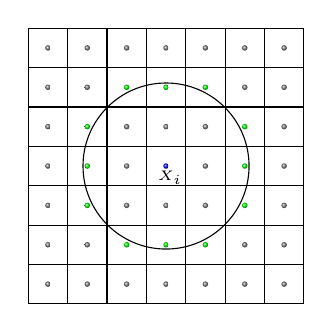
\begin{tikzpicture}
\shade[ball color = blue] (2,2) circle(1pt);
\shade[ball color = green] (1,1.5) circle(1pt);
\shade[ball color = green] (1,2.0) circle(1pt);
\shade[ball color = green] (1,2.5) circle(1pt);
\shade[ball color = green] (3,1.5) circle(1pt);
\shade[ball color = green] (3,2.0) circle(1pt);
\shade[ball color = green] (3,2.5) circle(1pt);
\shade[ball color = green] (1.5,1) circle(1pt);
\shade[ball color = green] (2.0,1) circle(1pt);
\shade[ball color = green] (2.5,1.) circle(1pt);
\shade[ball color = green] (1.5,3) circle(1pt);
\shade[ball color = green] (2.0,3) circle(1pt);
\shade[ball color = green] (2.5,3) circle(1pt);
 \foreach \x in {0.5,3.5}
 \foreach \y in {0.5,1,1.5,2,2.5,3,3.5}
 \shade[ball color = gray](\x,\y) circle (1pt);
 \foreach \x in {1,1.5,2,2.5,3}
 \foreach \y in {0.5,3.5}
 \shade[ball color = gray](\x,\y) circle (1pt);
 \foreach \x in {1.5,2,2.5}
 \foreach \y in {1.5,2.5}
 \shade[ball color = gray](\x,\y) circle (1pt);
 \foreach \x in {1,3}
 \foreach \y in {1,3}
 \shade[ball color = gray](\x,\y) circle (1pt);
 \shade[ball color = gray](1.5,2) circle (1pt);
 \shade[ball color = gray](2.5,2) circle (1pt);
 \foreach \x in {0.5,1,1.5,2,2.5,3,3.5,4.0}
 \draw(\x-0.25,0.25) -- (\x-0.25,4-0.25);
 \foreach \x in {0.5,1,1.5,2,2.5,3,3.5,4.0}
 \draw(0.25,\x-0.25) -- (4-0.25,\x-0.25);
 \draw(2,2) circle(30pt);
\node at (2.05,1.85) {\tiny{$X_i$}};
\end{tikzpicture}
\caption{Discrete mesh node $X_i$ on the equidistant grid and its interaction zone $B_\delta(X_i):=\lbrace X_j \vert \,\vert\vert X_j-X_i\vert\vert \leq \delta\rbrace$. }
\label{fig:emu}
\end{figure}

%----------------------------------------------------------------------------------------
\section{Algorithm}
%----------------------------------------------------------------------------------------
Figure~\ref{fig:algorithm:peri} shows the flow chart for the peridynamic simulation. The first step is to read the input file to obtain the material and discretization properties. Next, the discrete neighborhood for each of the nodes in computed and the neighbors are stored in a nested vector \cpp{std::vector<std::vector<size_t>>}. After these steps, the computation is started using a loop. Note that in the first computation the pair-wise forces $F$ are zero, since no external force $b$ was applied. In the next step, the external force $b$ is applied and the acceleration $a$ is computed. Note by adding the external force to the nodes, the acceleration of the nodes is not zero anymore. Now, the displacement $u$ is computed and the positions are updated. Last, the time step and time is updated.




\begin{figure}[tb]
    \centering
	\begin{tikzpicture}[node distance=1.125cm, scale=0.75, transform shape]
	\node (start) [startstop] {Start}; 
	\node (n0) [process, below of=start,yshift=-.5cm] {Read the input files};
	\node (n1) [process, below of=n0,yshift=-.5cm] {Compute the neighborhoods $B_\delta$~\eqref{eq:discrete:pd}};
	\node (dec1) [decision, below of=n1 , yshift=-1.cm] { $t_n < T$};
	\node (stop) [startstop, right of=dec1, xshift=3.cm] {Finished}; 
	\node (n4) [process, below of=dec1,yshift=-1.cm] {Compute the pair-wise force $f$~\eqref{eq:discrete:pd}};
	\node (n5) [process, below of=n4,yshift=-0.25cm] {Add external force $b$};
	\node (n6) [process, below of=n5,yshift=-0.25cm] {Compute the accerleration $a$~\eqref{eq:discrete:pd}};
	\node (n7) [process, below of=n6,yshift=-0.25cm] {Compute the displacement $u$~\eqref{eq:pd:displacement}};
	\node (n8) [process, below of=n7,yshift=-0.25cm] {Update the positions};
	\node (n9) [process, below of=n8,yshift=-0.25cm] { Update the time step $t_n = t_n + 1$};
	\node (n10) [process, below of=n9,yshift=-0.25cm] { Update the time $t=\Delta t * t_n$};
	%lines
	\draw [->] (start) -- (n0);
	\draw [->] (n0) -- (n1);
	\draw [->] (n1) -- (dec1);
	\draw [->] (dec1) -- node[anchor=north] {yes} (stop);
	\draw [->] (dec1) -- node[anchor=west] {no} (n4);
	\draw [->] (n4) -- (n5);	
	\draw [->] (n5) -- (n6);	
	\draw [->] (n6) -- (n7);	
	\draw [->] (n7) -- (n8);	
	\draw [->] (n8) -- (n9);	
	\draw [->] (n9) -- (n10);	
	\draw [->] (n10.west) -- ++(-3.0,0) -- ++(0,10.425) -- ++(4.25,0);
	\end{tikzpicture}
	\caption{Flow chart for the Peridynamic simulation.}
	\label{fig:algorithm:peri}
\end{figure}


%----------------------------------------------------------------------------------------
\chapter{One-dimensional heat equation}
%----------------------------------------------------------------------------------------
For the example for distributed computing, we look into the one-dimensional heat equation. The heat equation reads as
\begin{align}
\frac{\partial u}{\partial t} = \alpha \left( \frac{\partial^2 u }{\partial x^2} + \frac{\partial^2 u}{\partial y^2} + \frac{\partial^2 u}{\partial z^2} \right)
\label{eq:heat:full}
\end{align}
where $\alpha$ is the diffusivity of the material. The heat equation computes the flow of heat in a homogeneous and isotropic medium. For more details about the mathematics and physics of the heat equation, we refer to~\cite{cannon1984one}. For the distributed computing example, we look into the easiest case which is the one-dimensional heat equation. We assume a one-dimensional bar of length $L$ and Eqiation~\ref{eq:heat:full} reads as
\begin{align}
\frac{\partial u}{\partial t} = \alpha \frac{\partial^2 u}{\partial x^2}, \quad 0 \leq x \leq L, t >0.
\label{eq:heat:discrete}
\end{align}
To solve this one-dimensional heat equation, boundary conditions are required
\vspace{0.25cm}
\begin{itemize}
\item $u(0,t) = u_0$ 
\item $u(L,t) = u_L$
\item $u(x,0) = f_0(x)$.
\end{itemize}
\vspace{0.25cm}
First, a value at the beginning of the bar and at the end of the bar are given which are constant over time. For all other positions within the bar we apply an arbitrary value at time $t$ equal zero. However, to solve the heat equation from the numerical perspective, we have to discretize the equation in space and time. For the discretization in space a so-called discrete mesh 
\begin{align*}
x_i = (i-1) h, \quad i=1,2,\ldots,N
\end{align*}
where $N$ is the total number of nodes and h is given by $h=\sfrac{L}{N-1}$, see Figure~\ref{fig:heat:discrete:mesh}. The next step is to the discretization in time. Therefore, the approximation of the the second derivative $\sfrac{\partial^2 u}{\partial x^2}$ in Equation~\ref{eq:heat:discrete} using a central difference scheme. The first derivation reads as
\begin{align*}
\frac{\partial u}{\partial x} \approx \frac{u_{i+1}-u_{i}}{2h}
\end{align*}
and the second derivation reads as
\begin{align*}
\frac{\partial u}{\partial x^2} \approx \frac{u_{i-1}-2u_{i}+u_{i+1}}{2h}\text{.}
\end{align*}
Meaning we can approximate the second derivation at position $x_i$ using the left neighbor $x_{i-1}$ and the right neighbor $x_{i+1}$. Note that we do not have the left neighbor at $x_0$ and the right neighbor at $x_L$. Here, some special treatment is needed to compute the approximation of the derivation. To avoid this special treatment, we assume that we have a ring instead of a bar in our example. For more details about the finite difference method, we refer to~\cite{strikwerda2004finite,leveque2007finite}.
\begin{figure}[tb]
\center
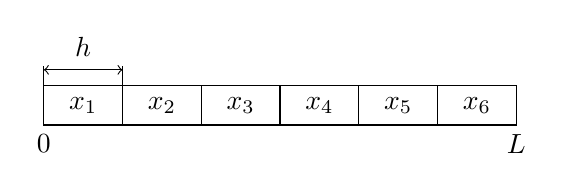
\begin{tikzpicture}
\draw(0,0) -- (6,0) -- (6,0.5) -- (0,0.5) -- cycle;
\node[below] at (0,0) {$0$};
\node[below] at (6,0) {$L$};
\foreach \i in {1,...,5}{
	\draw (\i,0) --(\i,0.5);	
}
\foreach \i in {1,...,6}{
	\node at (-0.5+\i,0.25) {$x_\i$};	
}
\draw (0,0.5) -- (0,0.75);
\draw (1,0.5) -- (1,0.75);
\draw[<->] (0,0.7) -- (1,0.7);
\node[above] at (0.5,0.75) {$h$};
\end{tikzpicture}
\caption{Discretization in space using a so--called discrete mesh for the one-dimensional heat equation.}
\label{fig:heat:discrete:mesh}
\end{figure}
Now, we combine the discretiztion on time and space, see Figure~\ref{fig:heat:time:space}, to compute the heat transfer for the next time step. At time $t=0$ we have applied the boundary conditions on the \textcolor{azure}{blue} squares. At time $t_i$ we compute the new value for the node $x_4$ at time $t_{i+1}$ using its neighbors's values at time $t_i$ using the central difference scheme. 

\begin{figure}[tb]
\center
\begin{tikzpicture}

\foreach \j in {1,...,5}{
\foreach \i in {1,...,6}{
	\node at (\i,\j) {\pgfuseplotmark{square*}};
}
}
\foreach \i in {1,...,6}{
	\node[color=azure] at (\i,0) {\pgfuseplotmark{square*}};
}
\foreach \i in {1,...,6}{
	\node[below] at (\i,-0.1) {$x_\i$};	
}

\draw[thick,->] (-1,0) -- (-.5,0);
\draw[thick,->] (-1,0) -- (-1,0.5);
\node[right] at (-0.5,0) {$x$};
\node[above] at (-1,0.5) {$t$};

\node[left] at (0.75,2) {$t_{i-1}$};
\node[left] at (0.75,3) {$t_{i}$};
\node[left] at (0.75,4) {$t_{i+1}$};

\node[below] at (1,-0.75) {$0$};
\node[below] at (6,-0.75) {$L$};

\draw (4,4) -- (4,3);
\draw (4,4) -- (3,3);
\draw (4,4) -- (5,3);
\end{tikzpicture}
\caption{Scheme for the discretization in space and time. At time $t=0$ the boundary conditions are applied at the \textcolor{azure}{squares}. We use the central difference scheme to compute the new values at time $t_{i+1}$ using the values from the previous time step. The central difference scheme is shown for the discrete mesh node $x_4$.}
\label{fig:heat:time:space}
\end{figure}

%----------------------------------------------------------------------------------------
\section{Serial implementation details}
%----------------------------------------------------------------------------------------
First, a function \cpp{heat} which implements the central difference scheme in Equation~\ref{eq:heat:discrete}, see Lines~10--13 in Listing~\ref{code:heat:central:difference}. Note that for simplicity we renamed $\alpha$ to $k$. We use the keyword \cpp{static} in front of the \cpp{return} type \cpp{double}. We will discuss later why we need to use the \cpp{static} keyword. The next step is to look into the data structure (partition) to store the heat values. For the serial implementation the partition is defined as \cpp{typedef double partition;} since we store one \cpp{double} value per discrete mesh node. For storing all heat values per discrete mesh node a \cpp{typedef std::vector<partition> space;} is declared. For the central difference scheme we need the heat values from the previous time step to compute the heat values for the current time step. So we need to have to \cpp{space} objects for both time steps, see Line~19 in Listing~\ref{code:heat:central:difference}. In Line~20--12 the size of the vector is set to the number of discrete mesh nodes $nx$. Since we have a nested vector \cpp{U[t][i]} the first index is the time step $t$ and the second one the index \cpp{i}. Thus to set the boundary conditions in Line~24--25 the first argument is zero for $t=0$ and we iterate over all discrete mesh nodes. \\

Since we have the initial setup, we can iterate over the time steps using the \cpp{for} loop in Line~28. Something tricky happens in Line~30--31 to swap the \cpp{space} for the current time step and the previous time step. Figure~\ref{fig:heat:swap} shows how to swap the \cpp{space} for each time step. For the initial time $t=0$ the space \cpp{U[0]} holds the current heat values and the space \cpp{U[1]} holds the heat values for the next time step $t=1$. To compute the heat values for the time step $t=2$ the space \cpp{U[0]} is reused to store the next heat values. For swapping the spaces, we use \cpp{t \% 2} to get the current space and \cpp{(t+1) \% 2} to get the space for the new heat values. Since we assume a ring, the computation of the first and last elements need a special treatment and all other points are computed the same. The complete source code for the serial example is available here\link{https://github.com/STEllAR-GROUP/hpx/blob/master/examples/1d_stencil/1d_stencil_1.cpp}. Choosing following boundary conditions 
\begin{align*}
u(x,0) = f(i,0), \text{ with } f(0,i)=i \text{ for } i=1,2,\ldots,N
\end{align*}
and a heat transfer coefficient $k$ = 0.5, time step size $dt$ = 1., grid spacing $h$ = 1., and time steps $nt$ = 45 results in the initial conditions, See Figure~\ref{fig::heat::initial}, and the solution, see Figure~\ref{fig::heat:solution}.

\begin{figure}[tb]
\centering
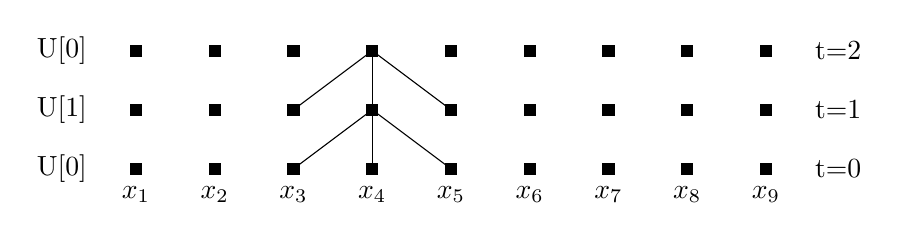
\begin{tikzpicture}

\foreach \i in {1,...,9}{
	\node[color=black] at (\i,1.5) {\pgfuseplotmark{square*}};
}

\foreach \i in {1,...,9}{
	\node[color=black] at (\i,0.75) {\pgfuseplotmark{square*}};
}


\foreach \i in {1,...,9}{
	\node[color=black] at (\i,0) {\pgfuseplotmark{square*}};
}
\foreach \i in {1,...,9}{
	\node[below] at (\i,-0.1) {$x_\i$};	
}

\node[left] at  (0.5,0) {U[0]};
\node[left] at  (0.5,0.75) {U[1]};
\node[left] at  (0.5,1.5) {U[0]};

\node[right] at  (9.5,0) {t=0};
\node[right] at  (9.5,0.75) {t=1};
\node[right] at  (9.5,1.5) {t=2};

\draw (3,0) -- (4,0.75);
\draw (4,0) -- (4,0.75);
\draw (5,0) -- (4,0.75);

\draw (3,0.75) -- (4,1.5);
\draw (4,0.75) -- (4,1.5);
\draw (5,0.75) -- (4,1.5);
\end{tikzpicture}
\caption{Sketch for swapping the partition to reuse the partition vectors to compute the new time step.}
\label{fig:heat:swap}
\end{figure}


\begin{figure}[bt]
\begin{subfigure}{.45\textwidth}
\centering
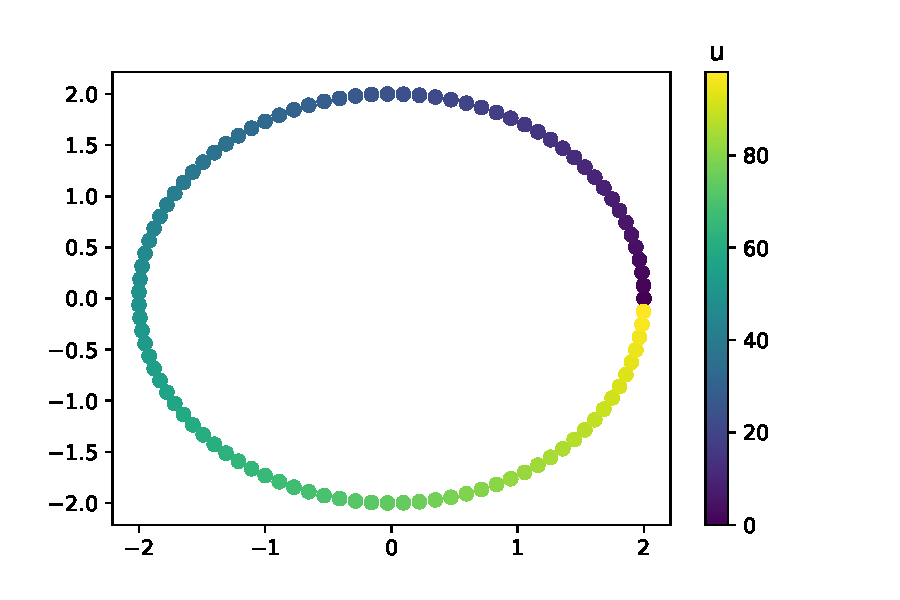
\includegraphics[width=\linewidth]{./images/initial_conditons.pdf}
\caption{Discrete nodes colored with their initial heat value prescribed by the boundary conditions.}
\label{fig::heat::initial}
\end{subfigure}
\hfill
\begin{subfigure}{.45\textwidth}
  \centering
  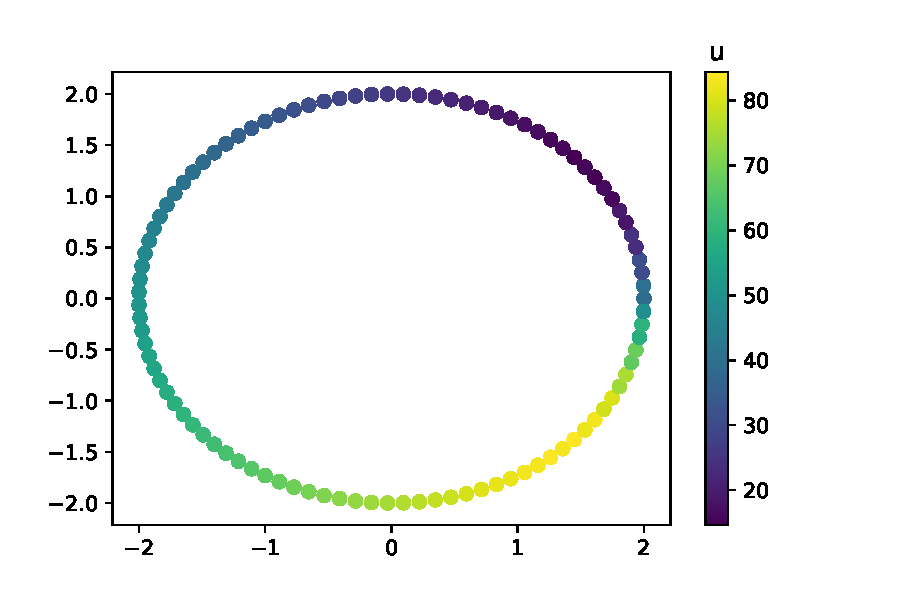
\includegraphics[width=\linewidth]{./images/solution.pdf}
\caption{Discrete nodes colored with final heat value at the final time $t=45$. }
\label{fig::heat:solution}
\end{subfigure}
\caption{The initial heat values prescribed by the boundary conditions~(\subref{fig::heat::initial}) and the final solution after 45 time steps~(\subref{fig::heat:solution}).}
\end{figure}


\begin{lstlisting}[language=c++,caption={Serial implementation of the one-dimensional heat equation \label{code:heat:central:difference}},float,floatplacement=tb]
struct stepper
{
    // Our partition type
    typedef double partition;

    // Our data for one time step
    typedef std::vector<partition> space;

    // Our operator
    static double heat(double left, double middle, double right)
    {
        return middle + (k*dt/(dx*dx)) * (left - 2*middle + right);
    }

    // do all the work on 'nx' data points for 'nt' time steps
    space do_work(std::size_t nx, std::size_t nt)
    {
        // U[t][i] is the state of position i at time t.
        std::vector<space> U(2);
        for (space& s : U)
            s.resize(nx);

        // Initial conditions: f(0, i) = i
        for (std::size_t i = 0; i != nx; ++i)
            U[0][i] = double(i);

        // Actual time step loop
        for (std::size_t t = 0; t != nt; ++t)
        {
            space const& current = U[t % 2];
            space& next = U[(t + 1) % 2];

            next[0] = heat(current[nx-1], current[0], current[1]);

            for (std::size_t i = 1; i != nx-1; ++i)
                next[i] = heat(current[i-1], current[i], current[i+1]);

            next[nx-1] = heat(current[nx-2], current[nx-1], current[0]);
        }

        // Return the solution at time-step 'nt'.
        return U[nt % 2];
    }
};
\end{lstlisting} 

%----------------------------------------------------------------------------------------
\subsection{Adding grain size control}
%----------------------------------------------------------------------------------------
In Figure~\ref{fig:hpx:stencil:scaling1} we have seen that we got some speedup with the asynchronous implementation discussed in Section~\ref{sec:hpx:advanced:sync}. However, in same cases the granularity (the amount of work) for each core was too small, since we always used one grid point wrapped in a future. Now, we want to extend the code to use partitions of grid nodes, see Figure~\ref{}. In this example we have a grid with nine nodes and we split them into three partitions, which means that each core has to compute the new values for three elements instead of for one element. The first, thing we need to do is to update the \cpp{struct participation}, see Listing~\ref{code:heat:garain:size}. In Line~4 a \cpp{std::vector<double>} is added to store the partition. In Line~8 a constructor is added to initialize the vector \cpp{data_(size)} with the provided \cpp{size_t size}. In Line~12 a second constructor is added to fill the partition with the initial values and the boundary values. Since the partition vector is declared as \cpp{private}, we use operator overloading in Line~21 and Line~25 to access the elements of the partition. For more details about operation overloading, see Section~\ref{sec:operator:overloading}. In Line~29 a function to obtain the partition size is added. \\

For the swapping scheme between the time steps for the computation of the temperature, see Figure~\ref{fig:heat:swap}, some small notification is applied as well. Figure~\ref{heat:swapping:partition} shows the principle of the swapping scheme using partitions. The fundamental principle is the same and we have the two space \cpp{U} to swap between the current time step and the future time step. However, with introducing the partitions, we have the two spaces per partition. These modifications are shown in Listing~\ref{code:heat:grain:size:stepper}. In Line~4 the \cpp{partition} is now of the type \cpp{partition_data}, see Listing~\ref{code:heat:garain:size}. In Line~10, each of the space vectors's size is set to the amount of partitions \cpp{np}. In Line~14, we access the space vector \cpp{U[0]} for the first time step and with \cpp{U[0][i]} each partition is accessed. We call the constructor for each partition and assign the initial values and boundary conditions. The full code is available on GitHub\link{https://github.com/STEllAR-GROUP/hpx/blob/master/examples/1d_stencil/1d_stencil_3.cpp}.


\begin{figure}[tp]
\centering
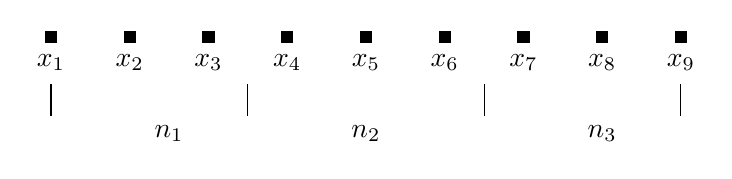
\begin{tikzpicture}

\foreach \i in {1,...,9}{
	\node at (\i,0) {\pgfuseplotmark{square*}};
}
\foreach \i in {1,...,9}{
	\node[below] at (\i,-0.1) {$x_\i$};	
}

\draw (1,-.6) -- (1,-1);
\draw (3.5,-.6) -- (3.5,-1);
\draw (6.5,-.6) -- (6.5,-1);
\draw (9,-.6) -- (9,-1);
\node[below] at (2.5,-1) {$n_1$};	
\node[below] at (5,-1) {$n_2$};	
\node[below] at (8,-1) {$n_3$};	
\end{tikzpicture}
\caption{Splitting the one-dimensional grid with nine grid nodes $(x_1,\ldots,x_9)$ into three partitions $(n_1,n_2,n3)$ to control the grain size.}
\end{figure}



\begin{lstlisting}[language=c++,caption={Serial implementation of the one-dimensional heat equation with grain size control. \label{code:heat:garain:size}},float,floatplacement=tbp]
struct partition_data
{


private:
    std::vector<double> data_;

public:

// Constructor
partition_data(std::size_t size = 0)
      : data_(size)
    {}

partition_data(std::size_t size, double int_value)
      : data_(size)
    {
        double base_value = 
              double(int_value * size);
        for (std::size_t i = 0; i != size; ++i)
            data_[i] = base_value + double(i);
    }

//Operator overloading 
double& operator[](std::size_t idx) { 
     return data_[idx]; 
  }
    
double operator[](std::size_t idx) const { 
       return data_[idx]; 
    }

// Util
std::size_t size() const { 
       return data_.size(); 
    }
};
\end{lstlisting}

\begin{figure}[tb]
\centering
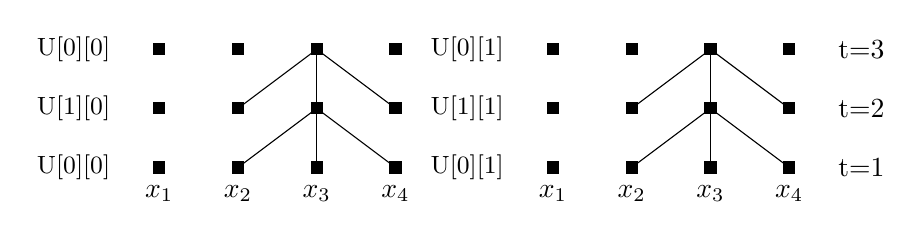
\begin{tikzpicture}

\foreach \j in {0,...,1}{


\foreach \i in {1,...,4}{
	\node at (\j*5+\i,1.5) {\pgfuseplotmark{square*}};
}

\foreach \i in {1,...,4}{
	\node at (\j*5+\i,0.75) {\pgfuseplotmark{square*}};
}


\foreach \i in {1,...,4}{
	\node at (\j*5+\i,0) {\pgfuseplotmark{square*}};
}
\foreach \i in {1,...,4}{
	\node[below] at (\j*5+\i,-0.1) {$x_\i$};	
}

\node[left] at  (\j*5+0.5,0) {\small U[0][\j]};
\node[left] at  (\j*5+0.5,0.75) {\small U[1][\j]};
\node[left] at  (\j*5+0.5,1.5) {\small U[0][\j]};

\draw (\j*5+2,0) -- (\j*5+3,0.75);
\draw (\j*5+3,0) -- (\j*5+3,0.75);
\draw (\j*5+4,0) -- (\j*5+3,0.75);

\draw (\j*5+2,0.75) -- (\j*5+3,1.5);
\draw (\j*5+3,0.75) -- (\j*5+3,1.5);
\draw (\j*5+4,0.75) -- (\j*5+3,1.5);

} 

\node[right] at  (9.5,0) {t=1};
\node[right] at  (9.5,0.75) {t=2};
\node[right] at  (9.5,1.5) {t=3};

\end{tikzpicture}
\caption{Swapping between the partitions using the two spaces \cpp{U}. Note that each partition $n$ has his dedicated spaces, however, the fundamental principle stays the same.}
\label{heat:swapping:partition}
\end{figure}



\begin{lstlisting}[language=c++,caption={Serial implementation of the one-dimensional heat equation with grain size control. \label{code:heat:grain:size:stepper}},float,floatplacement=tbp]
class stepper
{
    // Our data for one time step
    typedef partition_data partition;
    typedef std::vector<partition> space;
    
    std::vector<space> U(2);
    for (space& s: U)
        // np is the number of partitions
        s.resize(np);
        
    // Initial conditions: f(0, i) = i
    for (std::size_t i = 0; i != np; ++i)
        U[0][i] = partition_data(nx, double(i));
        
    // Return the solution at time-step 'nt'.
    return U[nt % 2];
    
}
\end{lstlisting}


\newpage
\theendnotes
